\chapter{Descrição do sistema}

O objetivo do presente trabalho é desenvolver um sistema capaz de posicionar um carro ao longo de uma guia linear. Esse sistema será doravante denominado posicionador linear. Sistemas similares são encontrados em diferentes aplicações reais, por exemplo, em impressoras a jato, o bico de deposição de tinta deve ser posicionado ao longo da trilha de impressão. A seguir, detalham-se as características do sistema construído, bem como os ensaios para a realização da modelagem do processo.

O posicionador linear é constituído por um carro que desliza sobre trilhos, permitindo apenas movimento em um grau de liberdade. O veículo é conectado a um motor CC (Corrente Contínua) por meio de uma correia. Dessa forma, converte-se a rotação do motor em movimento linear do carro. O protótipo completo é apresentado nas Figuras \ref{fig:vista_superior} e \ref{fig:vista_frontal}.

\begin{figure}[H]
    \centering
    \includegraphics[width=1\linewidth]{figuras/planta_vista_superior.png}
    \caption[Vista superior do posicionador linear]{Vista superior do posicionador linear.}
    \label{fig:vista_superior}
\end{figure}

\begin{figure}[H]
    \centering
    \includegraphics[width=1\linewidth]{figuras/planta_vista_frontal.jpg}
    \caption[Vista frontal do posicionador linear]{Vista frontal do posicionador linear.}
    \label{fig:vista_frontal}
\end{figure}

A estrutura é composta por duas guias lineares de 8 mm de diâmetro e 1 m de comprimento, essas são fixadas a uma tábua por meio de dois suportes para cada. O carro (feito usando impressão 3D) é conectado a essas guias por meio de dois rolamentos lineares. 

O motor é preso na tábua também por uma peça feita por impressão 3D. Para fixação da correia de transmissão, adotaram-se duas polias de 6 mm.

O controle da velocidade e do sentido de rotação do motor CC é realizado por meio de uma Ponte H. Especificamente, variando-se a tensão média e o sentido da corrente aplicados ao motor. No eixo do motor é conectado um \textit{encoder} incremental com quadratura, permitindo medir o deslocamento do carro a partir da posição inicial. Por fim, sensores de fim de curso são empregados para limitar a excursão do movimento do carro. A geração do sinal enviado à ponte H e as leituras da posição do veículo e dos sensores de fim de curso são realizadas utilizando um Arduino Mega, que também é empregado para embarcar a lei de controle.

Na sequência, detalham-se os módulos do posicionador linear desenvolvido.

\section{Sistema de atuação}
O motor CC adotado no trabalho é o JGB37-545B, apresentado na Figura \ref{fig:motor}. Como vantagens deste modelo, pode-se citar baixo custo de aquisição, boa relação torque-velocidade e baixa tensão de acionamento (12 V). 

\begin{figure}[H]
    \centering
    \includegraphics[width=0.5\linewidth]{figuras/motor.jpg}
    \caption[Motor modelo JGB37-545B]{Motor modelo JGB37-545B.}
    \label{fig:motor}
\end{figure}

O motor é alimentado por meio da Ponte H L298N, apresentada na Figura \ref{fig:ponteH}. O controle do sentido de giro do motor é realizado através de duas portas digitais da ponte H. A Tabela \ref{tab:pinos_ponte} mostra o estado de operação do motor de acordo com os níveis lógicos impostos a essas portas. Vale comentar que o nível lógico ``Falso'' está associado a um sinal de tensão de 0 V, enquanto que ``Verdadeiro'' é representado por um sinal de tensão de 5 V. 

\begin{figure}[H]
    \centering
    \includegraphics[width=0.3\linewidth]{figuras/L298N.jpg}
    \caption[Módulo driver ponte H L298N]{Módulo driver ponte H L298N \cite{L298N}.}
    \label{fig:ponteH}
\end{figure}

\begin{table}[H]
    \centering
    \caption[Estado de operação do motor de acordo com os níveis lógicos enviados às Portas 1 e 2 da Ponte H]{Estado de operação do motor de acordo com os níveis lógicos enviados às Portas 1 e 2 da Ponte H \cite{L298N}.}
    \begin{tabular}{c|c|c}
    \textbf{Porta} 1 & \textbf{Porta} 2 & \textbf{Estado} \\
    \hline
    Falso & Verdadeiro & Desligado \\
    Falso & Verdadeiro & Sentido horário \\
    Verdadeiro & Falso & Sentido anti-horário \\
    Verdadeiro & Verdadeiro & Freio \\
    \end{tabular}

    \label{tab:pinos_ponte}
\end{table}

O controle da velocidade do motor é realizado  por meio de um sinal PWM (\textit{Pulse Width Modulation}) gerado no Arduino. Esse tipo de sinal é uma onda quadrada com amplitude e frequência constantes e largura de pulso variável. Ao aplicar o PWM nos MOSFETs presentes na Ponte H, eles comutam na mesma frequência, dessa forma, a tensão média será proporcional ao \textit{duty cycle}, ou seja, o tempo que o sinal está ligado versus o tempo desligado em um determinado período de tempo \cite{morais2023implementaccao}. 

\section{Sensor de posição}
 Como já mencionado, acoplou-se um \textit{encoder} incremental no eixo do motor. Então, é possível medir tanto a velocidade quanto a posição angular do eixo do motor em relação à posição inicial. Sabendo que o deslocamento de um ponto na extremidade da polia é o mesmo que a do carro, torna-se possível medir o deslocamento do carro em relação à posição inicial. Em particular, o \textit{encoder} adotado gera 300 pulsos por rotação e a polia tem 6 mm de raio, tem-se uma precisão de aproximadamente 0,12 mm para a leitura da posição do carro.

\section{Sensor de fim de curso}
Com o intuito de evitar danos à estrutura do posicionador, foram anexados dois sensores de fim de curso com lógica NF  (Normalmente Fechado) em cada uma das extremidades da guia linear. A Figura \ref{fig:sensor_fim} contém uma foto de um sensor de fim de curso. Assim, uma medida de segurança é estabelecida para evitar a saída do carro do intervalo admissível de posição. Mais precisamente, sempre que um dos sensores é acionado, a alimentação do motor CC é interrompida.

 \begin{figure}[H]
    \centering
    \includegraphics[width=0.5\linewidth]{figuras/fim_de_curso.jpg}
    \caption[Sensor de Fim de Curso]{Sensor de Fim de Curso.}
    \label{fig:sensor_fim}
\end{figure}

\section{Microcontrolador}
Para embarcar o controlador do sistema, foi utilizado o microcontrolador Arduino Mega 2560 apresentado na Figura \ref{fig:conexoes}. O Arduino Mega possui 54 pinos digitais e 16 analógicos \cite{Arduino}. Esse controlador é baseado no ATmega2560, com 8 bits de arquitetura RISC avançada \cite{ATmega2560}. Detalhes sobre a memória desse microcontrolador encontram-se na Tabela \ref{tab:especificacoes}.

 \begin{figure}[H]
    \centering
    \includegraphics[width=0.6\linewidth]{figuras/sistema_atuador.jpg}
    \caption[Microcontrolador Arduino Mega]{Microcontrolador Arduino Mega.}
    \label{fig:conexoes}
\end{figure}

\begin{table}[H]
    \centering
    \caption[Especificações técnicas Arduino Mega 2560]{Arduino Mega 2560 \cite{ATmega2560}.}
    \begin{tabular}{c|c}
    \textbf{Arquitetura} & \textbf{AVR RISK avançada} \\
    \hline
    Memória FLASH & 256 Kb \\
    Memória EEPROM & 4 Kb \\
    Memória RAM & 8 Kb \\
    \end{tabular}
    \label{tab:especificacoes}
\end{table}

O Arduino Mega será utilizado para medir a posição do carro (utilizando o \textit{encoder}), controlar a velocidade e o sentido de giro do motor CC (utilizando a Ponte H) e receber os dados dos dois sensores de fim de curso.

O microcontrolador irá processar os dados e, com base na diferença entre as posições atual e desejada para o carro, calcular a ação de controle, no caso, a tensão média aplicada ao motor. Nota-se, portanto, que o sistema irá operar em malha fechada \cite{ogata2010engenharia}. Para projetar a lei de controle, realizou-se a modelagem matemática do sistema, como será descrito a seguir.

\section{Modelagem Matemática \label{modelagem}}
Para a realização da modelagem da dinâmica do posicionador linear, foi considerado o carro como um corpo rígido, ou seja, a distância entre quaisquer duas partes do corpo será sempre constante. A Figura \ref{fig:corpo_rigido} ilustra as forças atuantes sobre o corpo. Na imagem, a força exercida pelo motor é representada como $F_c$ e $F_a$ representa a força de atrito, $M$ é a massa do veículo.

 \begin{figure}[H]
    \centering
    \includegraphics[width=0.6\linewidth]{figuras/diagrama_forcas.png}
    \caption[Diagrama de forças do posicionador linear]{Diagrama de forças do posicionador linear.}
    \label{fig:corpo_rigido}
\end{figure}

Considerando que $x_c$ denota a posição do veículo em relação à posição inicial, utilizando a segunda lei de Newton, é possível escrever

\begin{equation}
    M\ddot{x}_c(t)=F_c(t)-F_a(t)
    \label{newton}
\end{equation}

Considerar-se-á que a relação entre a tensão média aplicada ao motor $V_M$ e a força $F_c$ é a seguinte:

\begin{equation}
    F_c(t)=K_aV_M(t)
    \label{atuacao}
\end{equation}

\noindent em que $K_a$ é uma constante do motor.

Também irá se supor que a força de atrito $F_a$ do sistema é dada pelo produto entre o coeficiente de atrito viscoso $B_c$ e a velocidade do carro $\dot{x}_c$. Matematicamente, 

\begin{equation}
    F_a(t)=B_c\dot{x}_c(t)
    \label{atrito}
\end{equation}

Inserindo \eqref{atuacao} e \eqref{atrito} em \eqref{newton}, tem-se que

\begin{equation}
    M\ddot{x}_c(t)=K_aV_M(t)-B_c\dot{x}_c(t)
    \label{newton2}
\end{equation}

Isolando $\ddot{x}_c$, obtém-se

\begin{equation}
    \ddot{x_c}=\frac{-B_c\dot{x}_c(t)}{M}+\frac{K_a}{M}V_m(t)
    \label{isolado}
\end{equation}

A Equação \eqref{isolado} é o modelo dinâmico entre a tensão média aplicada ao motor e a aceleração do carro. Tal modelo será adotado no projeto do controlador.

\subsection{Espaço de Estados}
Pode-se representar o sistema no espaço de estados. De forma genérica, um modelo no espaço de estados é descrito por \cite{ogata2010engenharia}

\begin{equation}
    P :\begin{cases} 
        \dot{X}(t) = AX(t) + BU(t) \\
        Y(t) = CX(t) + DU(t) \\
        \end{cases}
    \label{modelo_espaco_estados}
\end{equation}

\noindent sendo $X \in \mathbb{R}^{n_x}$ o vetor de estados, $U \in \mathbb{R}^{n_u}$ o vetor de controle e $Y \in \mathbb{R}^{n_y}$ as saídas do sistema. Mais ainda, $A$, $B$, $C$ e $D$ são matrizes do modelo com dimensões adequadas. Para o sistema dado por \eqref{isolado}, pode-se definir o vetor de estados como:

\begin{gather}
    X(t)= 
    \begin{bmatrix}
        X_1(t) \\ X_2(t) 
    \end{bmatrix}=
    \begin{bmatrix}
        x_c(t) \\ \dot{x}_c(t)
    \end{bmatrix}
    \label{vetor_estados}
\end{gather}

Já o vetor de controle é descrito como:

\begin{equation}
    U(t)=V_m(t)
    \label{vetor_controle}
\end{equation}

Assim, pode-se escrever o do posicionador linear no espaço de estados da seguinte forma:

\begin{gather}
    \begin{bmatrix}
        \dot{x}_c(t) \\ \ddot{x}_c(t)
    \end{bmatrix}=
    \begin{bmatrix}
        0 && 1 \\ 0 && -\frac{B_c}{M}
    \end{bmatrix}
    +
    \begin{bmatrix}
        x_c(t) \\ \dot{x}_c(t)
    \end{bmatrix}
    \begin{bmatrix}
        0 \\ \frac{K_a}{M}
    \end{bmatrix}
    Vm(t)
    \label{espaco_estados}
\end{gather}

\begin{gather}
    Y(t)=
    \begin{bmatrix}
        1 && 0
    \end{bmatrix}
    \begin{bmatrix}
        x_c(t) \\ \dot{x}_c(t)
    \end{bmatrix}
    \label{espaco_estados_saida}
\end{gather}

\subsection{Identificação dos parâmetros físicos}
\label{identificacao}

Foram realizados ensaios experimentais para identificar os parâmetros do sistema, sendo estes a massa do veículo $M$, o coeficiente de atrito viscoso $B_c$ e o ganho de atuação $K_a$. Para isso, foi definido $\dot{x}_c=v_c$. Dessa forma, reescreveu-se o modelo \eqref{isolado} em função da velocidade, obtendo a Equação \eqref{velocidade}. Um procedimento similar pode ser encontrado em \citeonline{netto2016relatorio}.

\begin{equation}
    \tau\dot{v}_c(t)+v_c(t)=k_0V_m(t)
    \label{velocidade}
\end{equation}

\noindent com

\begin{equation}
    \tau=\frac{M}{B_c},\;k_o=\frac{K_a}{B_c}
    \label{velocidade_parametros}
\end{equation}

Ao aplicar um degrau de tensão de amplitude $v_0$, a evolução da velocidade do carro será dada por \cite{ogata2010engenharia} 

\begin{equation}
    v_c(t)=k_0v_0(1-e^\frac{-t}{\tau})
    \label{equacao_ordem1}
\end{equation}

Os coeficientes desconhecidos $\tau$ e $k_0$ podem ser facilmente identificados com base na resposta experimental ao degrau. Mais precisamente, ao aplicar um degrau de tensão de amplitude conhecida $v_0$, a velocidade em regime permanente tenderá para $k_0v_0$.
O instante de tempo em que $v_c$ atingir 63\% do seu valor de regime permanente é a constante de tempo $\tau$.

Seguindo essa metodologia, foram realizados ensaios com amplitudes de degrau de tensão diferentes. No instante $t = 0$~s, com o carro em repouso, aplicaram-se tais entradas e mediu-se a evolução temporal da velocidade. Foi observado que, para amplitudes menores que 3 V, o motor não consegue exercer força suficiente para movimentar o sistema, em virtude do do atrito seco no conjunto e da zona morta do motor CC. Tal efeito prático será incluído nas simulações do processo. 

As Figuras \ref{fig:resp_degrau3}--\ref{fig:resp_degrau12} apresentam a resposta da velocidade para os degraus de amplitudes 3, 6, 9 e 12 V. Vale comentar que a velocidade medida foi filtrada utilizando um filtro Butterworth digital de segunda ordem. Os detalhes de projeto desse filtro encontram-se no Apêndice \ref{apend:1}.

\begin{figure}[H]
    \centering
    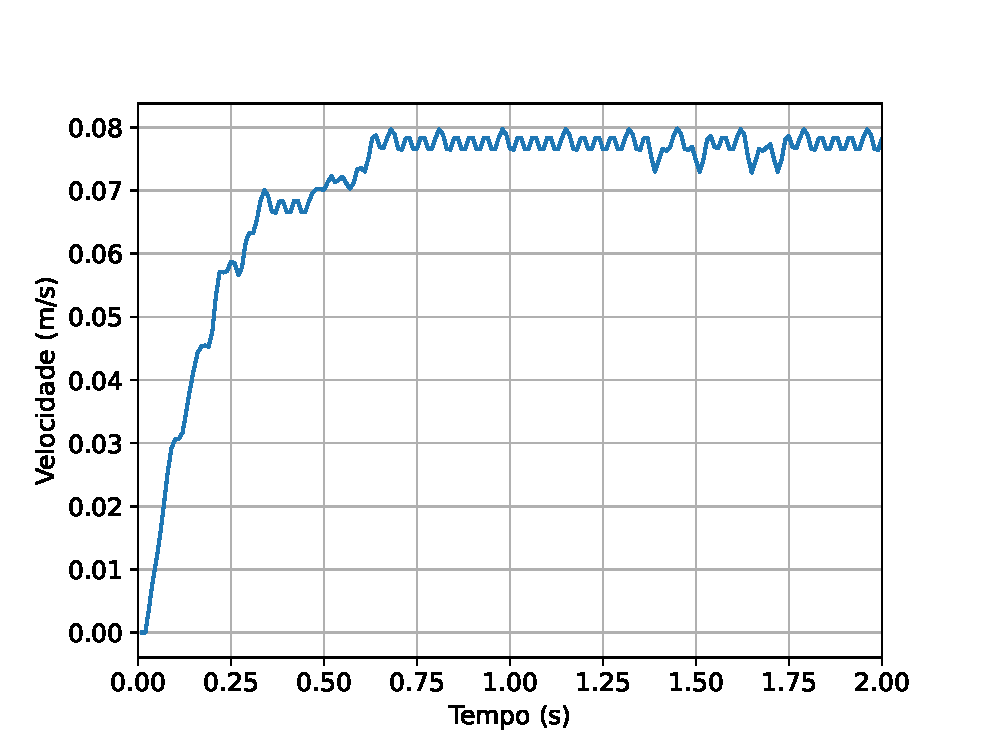
\includegraphics[width=0.8\linewidth]{figuras/degrau_3V.eps}
    \caption[Resposta de velocidade do carro para o degrau de tensão de amplitude 3 V]{Resposta de velocidade do carro para o degrau de tensão de amplitude 3 V.}
    \label{fig:resp_degrau3}
\end{figure}

\begin{figure}[H]
    \centering
    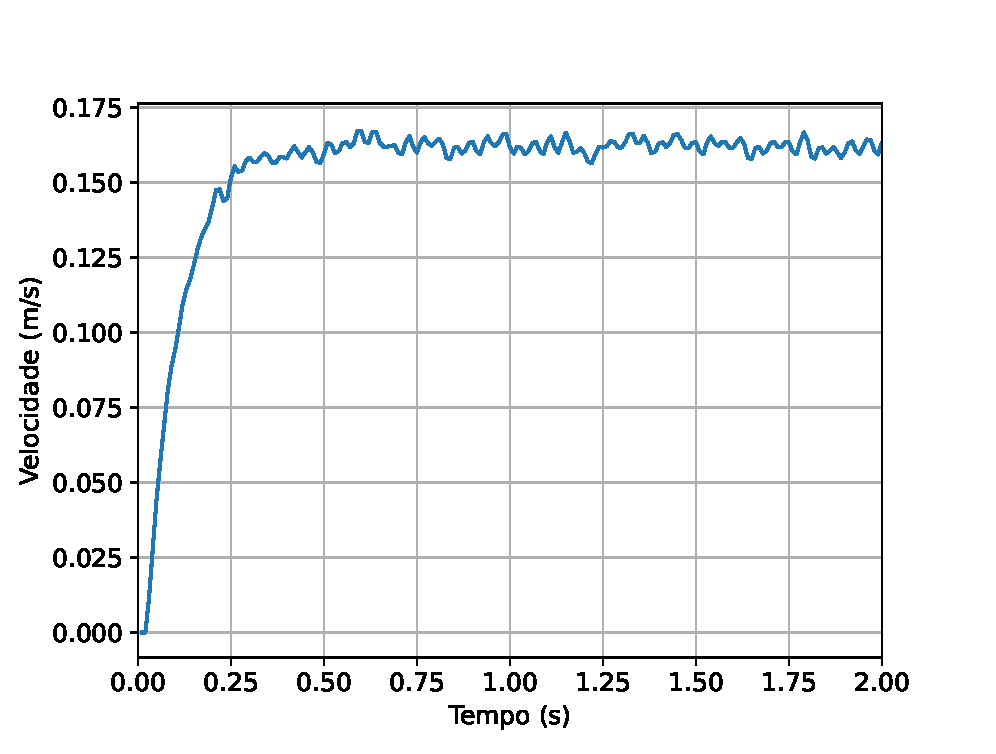
\includegraphics[width=0.8\linewidth]{figuras/degrau_6V.eps}
    \caption[Resposta de velocidade do carro para o degrau de tensão de amplitude 6 V]{Resposta de velocidade do carro para o degrau de tensão de amplitude 6 V.}
    \label{fig:resp_degrau6}
\end{figure}

\begin{figure}[H]
    \centering
    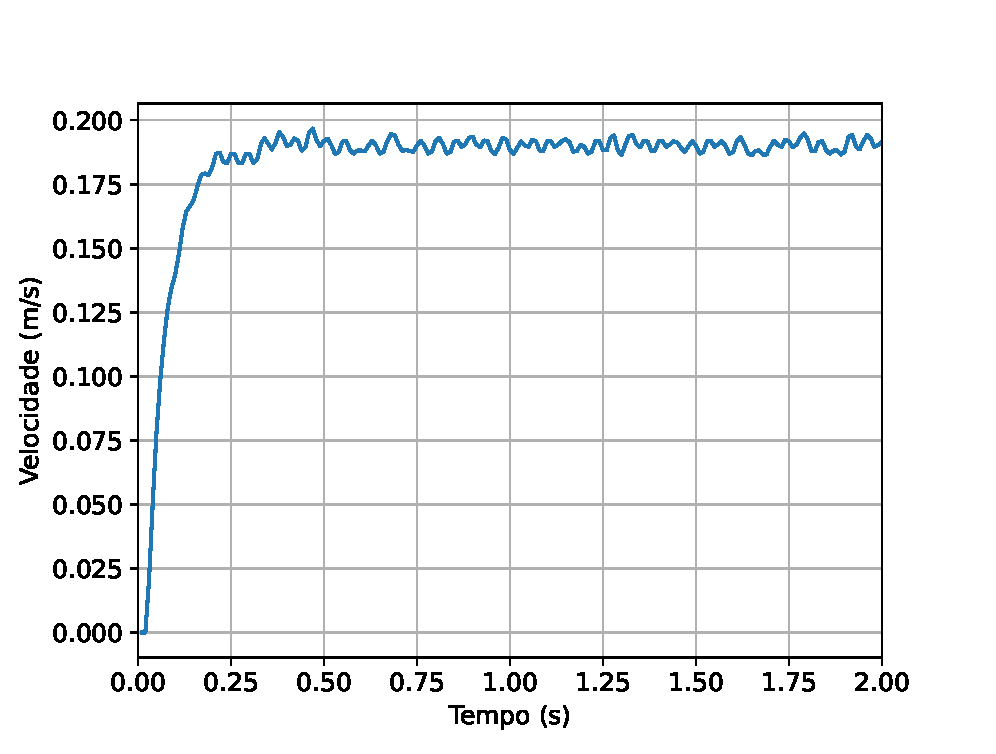
\includegraphics[width=0.8\linewidth]{figuras/degrau_9V.eps}
    \caption[Resposta de velocidade do carro para o degrau de tensão de amplitude 9 V]{de velocidade do carro para o degrau de tensão de amplitude 9 V.}
    \label{fig:resp_degrau9}
\end{figure}

\begin{figure}[H]
    \centering
    \includegraphics[width=0.8\linewidth]{figuras/degrau_12V.eps}
    \caption[Resposta de velocidade do carro para o degrau de tensão de amplitude 12 V.]{Resposta de velocidade do carro para o degrau de tensão de amplitude 12 V.}
    \label{fig:resp_degrau12}
\end{figure}

Com os dados obtidos, foi realizada a identificação dos parâmetros $\tau$ e $k_0$ para cada um dos degraus de tensão. Os resultados estão apresentados na Tabela \ref{tab:parametros_identificados}.

\begin{table}[H]
    \centering
    \caption[Parâmetros identificados]{Parâmetros identificados.}
    \begin{tabular}{c|c|c}
    \textbf{Tensão (V)} & \bm{$\tau$} \textbf{(s)} & \bm{$k_0 \mathrm{(\frac{rad}{Vms})}$}\\ [2pt] 
    \hline
    3 & 5,93 & 0,1512  \\
    6 & 10,69 & 0,2888 \\
    9 & 15,89 & 0,3364 \\
    12 & 22,24 & 0,3955 \\
    \end{tabular}
    \label{tab:parametros_identificados}
\end{table}

Pode-se constatar que os parâmetros do sistema mudam conforme a amplitude do degrau de tensão é variada. Isso indica a presença de não linearidades (possivelmente associadas com o atrito seco e zona morta).

Observando \eqref{velocidade_parametros}, nota-se que, apenas com os valores de $\tau$ e $k_0$, não é possível calcular os parâmetros do modelo ($M$, $M_c$ e $K_a$). Isso ocorre pois têm-se duas equações e três variáveis. Para resolver o problema foi realizado um ensaio adicional apenas para identificação de $K_a$.

\subsection{Identificação do ganho de atuação}
Com esse intuito, foi feita uma nova montagem, o motor foi retirado da correia e foi fixada uma haste de 0,5 m de comprimento e massa desprezível em seu eixo. Na extremidade livre dessa haste foi acoplada uma massa de 0,3 kg. Com a haste inicialmente em repouso na posição inferior, ao se aplicar um nível de tensão, o motor exercerá um torque $T$ em um sentido, enquanto que o peso $P$ da massa exercerá um momento no sentido contrário, a medida que o ângulo com o eixo vertical $\theta$ aumenta, o momento realizado pelo peso também irá aumentar, até chegar um ponto em que o sistema estabilize. Isto é que $T = P$. Para ilustrar a ideia, a Figura \ref{fig:diagrama_torque} representa o diagrama de forças do ensaio.

\begin{figure}[H]
    \centering
    \includegraphics[width=0.2\linewidth]{figuras/diagrama_torque.png}
    \caption[Diagrama de forças do ensaio do motor]{Diagrama de forças do ensaio do motor.}
    \label{fig:diagrama_torque}
\end{figure}

Estando o sistema em equilíbrio, pode-se escrever

\begin{equation}
    T = \text{sen}(\theta)mgd
    \label{torque_motor}
\end{equation}

\noindent em que $d = 0,5$~m é o comprimento da haste.

Seguindo a metodologia descrita, foi realizado o ensaio para diferentes níveis de tensão, o resultado é apresentado na Tabela \ref{tab:ensaio_motor}.

\begin{table}[H]
    \centering
    \caption[Resultados do ensaio de torque do motor]{Resultados do ensaio de torque do motor.}
    \begin{tabular}{c|c|c}
    \textbf{Tensão (V)}  & \bm{$\theta$} \textbf{(º)} & \textbf{Torque $T$ (Nm)}\\ \hline
    0 & 0 & 0,00 \\ 
    3 & 7 & 0,18 \\ 
    4 & 8 & 0,20 \\ 
    5 & 10 & 0,26 \\ 
    6 & 11 & 0,28 \\ 
    7 & 15 & 0,38 \\ 
    8 & 18 & 0,45 \\ 
    9 & 20 & 0,50 \\ 
    10 & 22 & 0,55 \\ 
    11 & 23 & 0,57 \\ 
    12 & 27 & 0,67 \\ 
    \end{tabular}
    \label{tab:ensaio_motor}
\end{table}

Considerando que $F_a = T/r$, é possível reescrever \eqref{torque_motor} do seguinte modo:

\begin{equation}
    K_aV_m = \underbrace{\text{sen}(\theta)\frac{mgd}{r}}_{\text{Força Motor}}
    \label{forca_motor}
\end{equation}

\noindent sendo $r=6$~mm o raio da polia.

Nota-se que existe uma relação linear entre a tensão média $V_m$ e a divisão do momento da força peso pelo raio da roldana. Assim, ao realizar uma regressão linear com esses dados, o coeficiente angular obtido será igual ao ganho de atuação. Após realizada, foi obtido um valor de 9,1898 N/V
para $K_a$, a Figura \ref{fig:regressao} apresenta a comparação entre os resultados experimentais e a regressão linear.

\begin{figure}[H]
    \centering
    \includegraphics[width=0.8\linewidth]{figuras/regressao.eps}
    \caption[Comparação entre resultados experimentais e regressão linear para identificação de $K_a$]{Comparação entre resultados experimentais e regressão linear para identificação de $K_a$.}
    \label{fig:regressao}
\end{figure}

Conhecendo-se $K_a$ e os dados da Tabela \ref{tab:parametros_identificados}, pode-se utilizar \eqref{velocidade_parametros} para obter os valores do coeficiente de $B_c$ e $M$ (vide Tabela \ref{tab:parametros_calculados}).

\begin{table}[H]
    \centering
    \caption[Valores de $B_c$ e $M$ para as diferentes amplitudes de degrau]{Valores de $B_c$ e $M$ para as diferentes amplitudes de degrau.}
    \begin{tabular}{c|c|c|c|c}
    \textbf{Tensão (V)} & \bm{$\tau$} \textbf{(s)} & \bm{$k_0 \mathrm{(\frac{rad}{Vms}})$} & \bm{$B_c \mathrm{(\frac{Ns}{m^2})}$} & \textbf{M (kg)}\\[3pt]  \hline
    3 & 0,15 & 5,93 & 60,78 & 10,25 \\ 
    6 & 0,29 & 10,69 & 31,82 & 2,98 \\ 
    9 & 0,34 & 15,89 & 27,32 & 1,72 \\ 
    12 & 0,40 & 22,24 & 23,24 & 1,04 \\ 
     &  & Média & 35,79 & 4,00 \\                  
    \end{tabular}
    \label{tab:parametros_calculados}
\end{table}

É possível constatar que os valores determinador para tensão de 3 V se distanciam dos demais. Isso pode estar associado com a forte presença do atrito para essa faixa de tensão. Entretanto, os resultados para tal amplitude de entrada não foram desconsiderados, tendo em vista que caso o sistema opere em tal condição, o modelo será mais representativo. Sendo assim, no projeto do controlador adotou-se a média dos parâmetros.

\subsection{Validação do modelo teórico}
Para validar o modelo levantado, aplicou-se no equipamento real e em simulação entradas iguais e comparam-se as respostas (i.e. o movimento do carro). 

Para implementação da simulação computacional, foi utilizada a função \textit{odeint} da biblioteca \textit{scipy}, cuja a documentação pode ser encontrada em \url{https://docs.scipy.org/doc/scipy/reference/generated/scipy.integrate.odeint.html}. Essa função foi utilizada para integrar numericamente o modelo matemático do sistema dado por \eqref{espaco_estados} e considerando a média dos parâmetros encontrados.

Em particular, as entradas foram ondas quadradas com amplitudes 3 V, 6 V, 9 V e 12 V, com frequências 0,25 Hz, 0,5 Hz, 1 Hz e 1 Hz, respectivamente. O sistema foi submetido a essas ondas por 8 segundos. As Figuras \ref{fig:validacao_3V}--\ref{fig:validacao_12V} apresentam a comparação entre as respostas experimental e simulada em cada um dos cenários descritos.

Pode-se notar que o modelo representou adequadamente o comportamento do sistema físico, possibilitando utilizá-lo projetar o controlador, como será descrito no capítulo a seguir.

\begin{figure}[H]
    \centering
    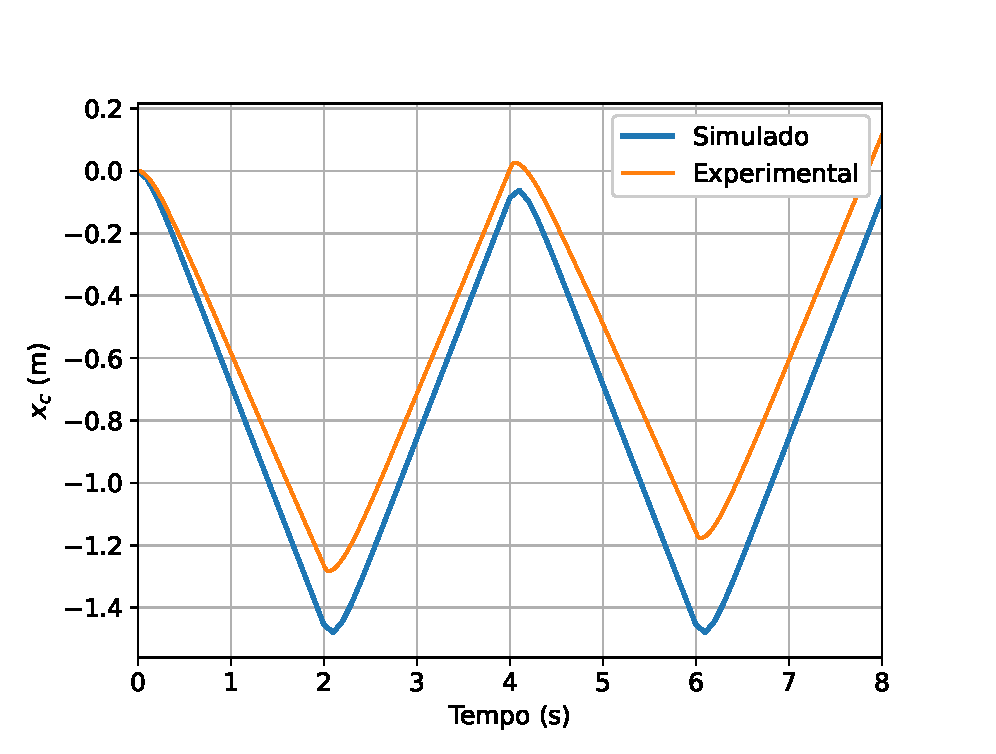
\includegraphics[width=0.8\linewidth]{figuras/validacao_3V.eps}
    \caption[Comparação entre as respostas simulada e experimental a uma onda quadrada com 3~V de amplitude e 0,25~Hz de frequência]{Comparação entre as respostas simulada e experimental a uma onda quadrada com 3~V de amplitude e 0,25~Hz de frequência.}
    \label{fig:validacao_3V}
\end{figure}

\begin{figure}[H]
    \centering
    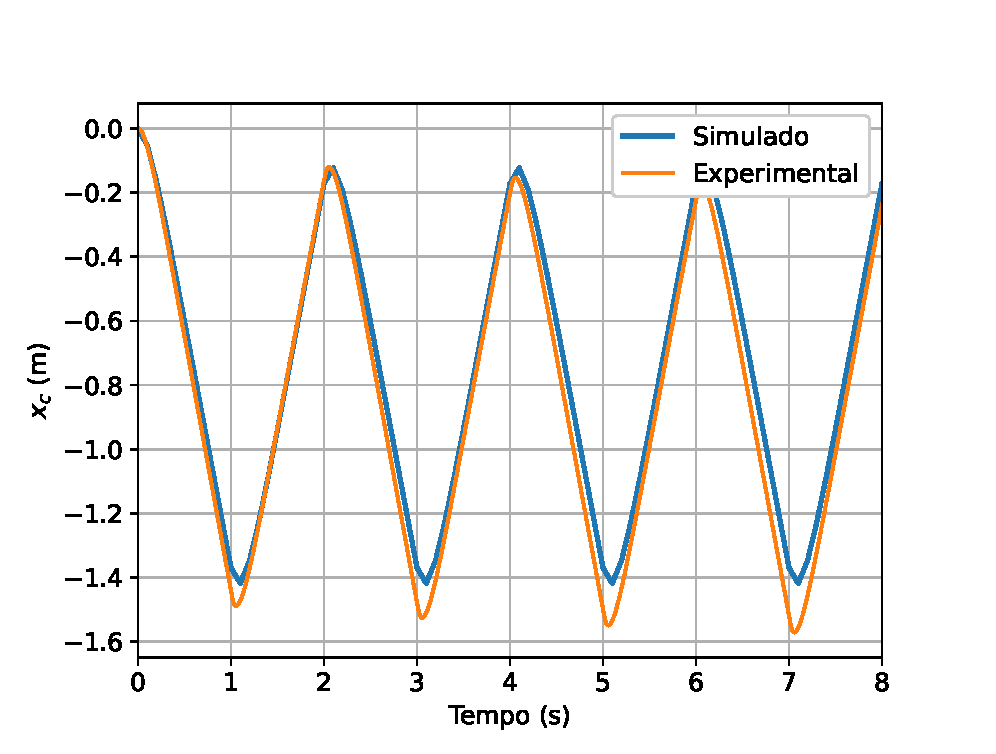
\includegraphics[width=0.8\linewidth]{figuras/validacao_6V.eps}
    \caption[Comparação entre as respostas simulada e experimental a uma onda quadrada com 6~V de amplitude e 0,5~Hz de frequência]{Comparação entre as respostas simulada e experimental a uma onda quadrada com 6~V de amplitude e 0,5~Hz de frequência.}
    \label{fig:validacao_6V}
\end{figure}

\begin{figure}[H]
    \centering
    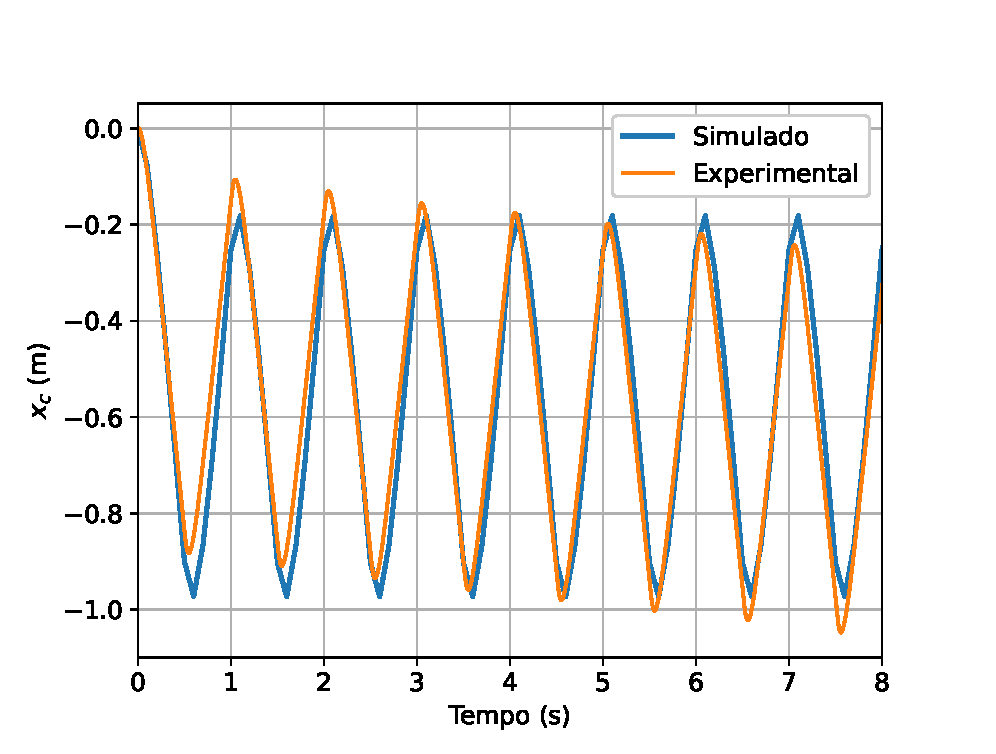
\includegraphics[width=0.8\linewidth]{figuras/validacao_9V.eps}
    \caption[Comparação entre as respostas simulada e experimental a uma onda quadrada com 9~V de amplitude e 1~Hz de frequência]{Comparação entre as respostas simulada e experimental a uma onda quadrada com 9~V de amplitude e 1~Hz de frequência.}
    \label{fig:validacao_9V}
\end{figure}

\begin{figure}[H]
    \centering
    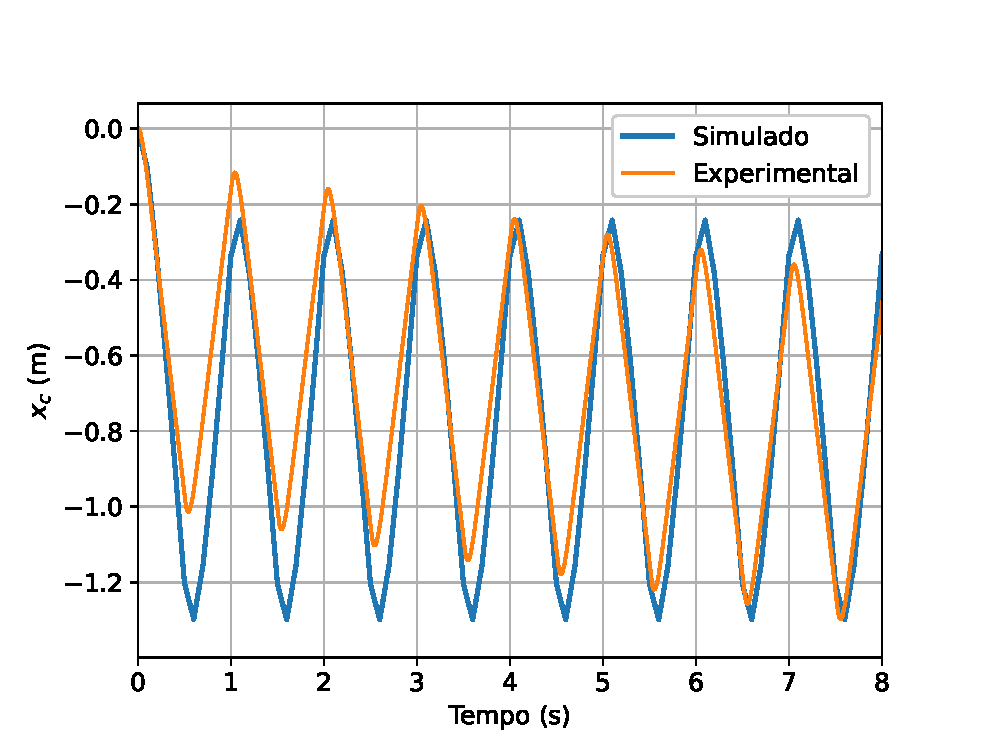
\includegraphics[width=0.8\linewidth]{figuras/validacao_12V.eps}
    \caption[Comparação entre as respostas simulada e experimental a uma onda quadrada com 12~V de amplitude e 1~Hz de frequência]{Comparação entre as respostas simulada e experimental a uma onda quadrada com 12~V de amplitude e 1~Hz de frequência.}
    \label{fig:validacao_12V}
\end{figure}
